%%%%%%%%%%%%%%%%%%%%%%%%%%%%%%%%%%%%%%%%%%%%%%%%%%%%%%%%%%%%%%%%%%%%%%%%%%%%%%%%%%%%%%
% Modelo de relatório de Disciplina de MLP a partir da
% classe latex iiufrgs disponivel em http://github.com/schnorr/iiufrgs
%%%%%%%%%%%%%%%%%%%%%%%%%%%%%%%%%%%%%%%%%%%%%%%%%%%%%%%%%%%%%%%%%%%%%%%%%%%%%%%%%%%%%%

% Ignore o comentario acima e imagine que exista um modelo de relatorio de CCI em algum lugar

%%%%%%%%%%%%%%%%%%%%%%%%%%%%%%%%%%%%%%%%%%%%%%%%%%%%%%%%%%%%%%%%%%%%%%%%%%%%%%%%%%%%%%
% Definição do tipo / classe de documento e estilo usado
%%%%%%%%%%%%%%%%%%%%%%%%%%%%%%%%%%%%%%%%%%%%%%%%%%%%%%%%%%%%%%%%%%%%%%%%%%%%%%%%%%%%%%
%
\documentclass{iiufrgs}

%%%%%%%%%%%%%%%%%%%%%%%%%%%%%%%%%%%%%%%%%%%%%%%%%%%%%%%%%%%%%%%%%%%%%%%%%%%%%%%%%%%%%%
% Importação de pacotes
%%%%%%%%%%%%%%%%%%%%%%%%%%%%%%%%%%%%%%%%%%%%%%%%%%%%%%%%%%%%%%%%%%%%%%%%%%%%%%%%%%%%%%
% (a A seguir podem ser importados os pacotes necessários para o documento, de acordo 
% com a necessidade)
%
\usepackage[brazilian]{babel}	    % para texto escrito em pt-br
\usepackage[utf8]{inputenc}         % pacote para acentuação
\usepackage{graphicx}         	    % pacote para importar figuras
\usepackage[T1]{fontenc}            % pacote para conj. de caracteres correto
\usepackage{times}                  % pacote para usar fonte Adobe Times
\usepackage{enumerate}              % para lista de itens com letras
\usepackage{breakcites}
\usepackage{tikz}
\usepackage[oldvoltagedirection]{circuitikzgit}
\usepackage{caption}
\usepackage{siunitx}
\usepackage{placeins}
\usepackage{titlesec}
\usepackage{enumitem}
\usepackage{titletoc}
\usepackage{subfig}
%\usepackage{listings}			    % para listagens de código-fonte
\usepackage{mathptmx}               % p/ usar fonte Adobe Times nas formulas matematicas
\usepackage{url}                    % para formatar URLs
%\usepackage{color}				    % para imagens e outras coisas coloridas
\usepackage{fixltx2e}              % para subscript
%\usepackage{amsmath}               % para \epsilon e matemática
%\usepackage{amsfonts}
%\usepackage{setspace}			    % para mudar espaçamento dos parágrafos
%\usepackage[table,xcdraw]{xcolor}  % para tabelas coloridas
%\usepackage{longtable}             % para tabelas compridas (mais de uma página)
%\usepackage{float}
%\usepackage{booktabs}
\usepackage{tabularx}
%\usepackage{hyperref}

\usepackage[alf,abnt-emphasize=bf]{abntex2cite}	% pacote para usar citações abnt

%%%%%%%%%%%%%%%%%%%%%%%%%%%%%%%%%%%%%%%%%%%%%%%%%%%%%%%%%%%%%%%%%%%%%%%%%%%%%%%%%%%%%%
% Macros, ajustes e definições
%%%%%%%%%%%%%%%%%%%%%%%%%%%%%%%%%%%%%%%%%%%%%%%%%%%%%%%%%%%%%%%%%%%%%%%%%%%%%%%%%%%%%%
%

% define estilo de parágrafo para citação longa direta:
\newenvironment{citacao}{
    %\singlespacing
    %\footnotesize
    \small
    \begin{list}{}{
        \setlength{\leftmargin}{4.0cm}
        \setstretch{1}
        \setlength{\topsep}{1.2cm}
        \setlength{\listparindent}{\parindent}
    }
    \item[]}{\end{list}
}

% adiciona a fonte em figuras e tabelas
\newcommand{\fonte}[1]{\\Fonte: {#1}}

\newcommand{\virtuoso}{\textit{Virtuoso}}

\newcommand{\titlepagespecificinfo}{Relatório apresentado como requisito parcial para a obtenção de conceito na Disciplina de Concepção de Circuitos Integrados.}
% \def\@cipspecificinfo{Concepção de Circuitos Integrados}


% Ative o seguinte caso alguma nota de rodapé fique muito longa e quebre entre múltiplas
% páginas
%\interfootnotelinepenalty=10000

%%%%%%%%%%%%%%%%%%%%%%%%%%%%%%%%%%%%%%%%%%%%%%%%%%%%%%%%%%%%%%%%%%%%%%%%%%%%%%%%%%%%%%
% Informações gerais                                   
%%%%%%%%%%%%%%%%%%%%%%%%%%%%%%%%%%%%%%%%%%%%%%%%%%%%%%%%%%%%%%%%%%%%%%%%%%%%%%%%%%%%%%

% título
\title{RELATÓRIO 5} 

% autor
%\author{Autores(s)}{Aluno(s)} % {sobrenome}{nome}
\author{Silva}{Henrique Corrêa Pereira da}

% Professor orientador da disciplina
\advisor[Prof.~Dr.]{Augusto da Luz Reis}{Ricardo}

% Nome do(s) curso(s):
\course{Curso de Graduação em Ciência da Computação}

% local da realização do trabalho 
\location{Porto Alegre}{RS} 

% data da entrega do trabalho (mês e ano)
\date{7}{2018}


% Palavras chave
\keyword{CCI}
\keyword{Virtuoso}
\keyword{Somador}
\keyword{Relatório}


%%%%%%%%%%%%%%%%%%%%%%%%%%%%%%%%%%%%%%%%%%%%%%%%%%%%%%%%%%%%%%%%%%%%%%%%%%%%%%%%%%%%%%
% Início do documento e elementos pré-textuais
%%%%%%%%%%%%%%%%%%%%%%%%%%%%%%%%%%%%%%%%%%%%%%%%%%%%%%%%%%%%%%%%%%%%%%%%%%%%%%%%%%%%%%

% Declara início do documento
\begin{document}

% inclui folha de rosto 
\maketitle

\selectlanguage{brazilian}

% Sumario
\tableofcontents



%%%%%%%%%%%%%%%%%%%%%%%%%%%%%%%%%%%%%%%%%%%%%%%%%%%%%%%%%%%%%%%%%%%%%%%%%%%%%%%%%%%%%
% Aqui comeca o texto propriamente dito
%%%%%%%%%%%%%%%%%%%%%%%%%%%%%%%%%%%%%%%%%%%%%%%%%%%%%%%%%%%%%%%%%%%%%%%%%%%%%%%%%%%%%

%espaçamento entre parágrafos
%\setlength{\parskip}{6 pt}

\selectlanguage{brazilian}

%%%%%%%%%%%%%%%%%%%%%%%%%%%%%%%%%%%%%%%%%%%%%%%%%%%%%%%%%%%%%%%%%%%%%%%%%%%%%%%%%%%%%
% Visao Geral
%

\chapter{Introdução}\label{intro}

Como definido no plano de ensino da disciplina, este relatório abordará o desenvolvimento do trabalho final da disciplina, um Somador de 4 bits \textit{mirror-adder ripple carry} com \textit{carry-in} e \textit{carry-out}. Sendo assim, analisaremos sua performance utilizando as seguintes métricas:

\begin{enumerate}[leftmargin=3em, noitemsep] % [label={--}]
    \setlength{\itemindent}{1em}
    \item T\textsubscript{lh}: tempo de subida do sinal;
    \item T\textsubscript{hl}: tempo de descida do sinal;
    \item Tp\textsubscript{lh}: tempo de propagação \textit{low-low}; 
    \item Tp\textsubscript{hl}: tempo de propagação \textit{high-high}; 
    \item Tp\textsubscript{médio}: tempo de propagação médio; 
    \item P\textsubscript{média}: potência média das células; 
    \item P\textsubscript{RMS}: potência \textit{RMS} das células;
    \item Área: área ocupada pelo layout final.
\end{enumerate}

Além disso, será feita a análise \textit{Layout versus Schematic} para a célula a fim de  verificar a funcionalidade do leiaute contra o esquemático. Mais detalhes sobre a implementação do circuito de lógica sequencial e do circuito elétrico em si no Capítulo \nameref{proposta}.

\begin{figure}[htb]
    \centering
    \caption{Circuito do somador de 4 bits \textit{mirror-adder ripple carry} a ser projetado.}
    \label{fig:4bit_pretty}
    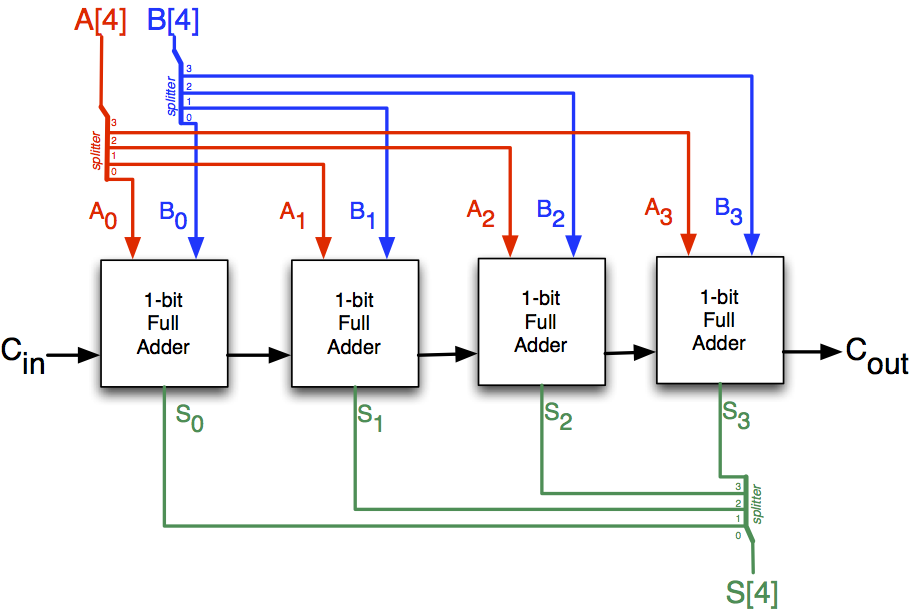
\includegraphics[scale=0.65]{images/pretty.png}
\end{figure}

\chapter{Proposta}\label{proposta}
A proposta do relatório é construir e realizar a medição de métricas de implementações do \textbf{Somador de 4 bits} na tecnologia CMOS C35B4 da \textit{Austria Microsystems}, utilizando valores de W\textsubscript{p} e de W\textsubscript{n} dessas respectivas portas conforme a Tabela \ref{tab:imp} e uma lógica de transistores de passagem.
Além disso, o circuito também deverá seguir às seguintes especificações:

\begin{itemize}[noitemsep]
    \setlength{\itemindent}{1em}
    \item VDD = \SI{3.3}{\V};
    \item Duração das simulações transiente = \SI{30}{\ns};
    \item Tinput\textsubscript{rise} = \SI{100}{\ps};
    \item Tinput\textsubscript{fall} = \SI{100}{\ps}.
\end{itemize}

Criados os leiautes, é obrigatório tanto o teste individual utilizando as ferramentas \textit{DRC} e \textit{LVS} quanto a extração das capacitâncias parasitas das implementações.

\begin{table}[ht]
    \centering
    \caption{Dimensões das implementações.}
    \label{tab:imp}
    \begin{tabular}{l c c}
        \hline
        Implementação
        & W\textsubscript{p}
        & W\textsubscript{n} \\ \hline
        Inversor        & \SI{4.2}{\um}                 & \SI{2.6}{\um}                  \\
        Somador 1 bit   & \SI{4.2}{\um} e \SI{2.1}{\um} & \SI{2.6}{\um} e \SI{1.3}{\um}  \\ \hline
    \end{tabular}
\end{table}

Como podemos observar na Tabela \ref{tab:imp}, o Somador de 1 bit utiliza dois tamanhos de transistores W\textsubscript{p} e W\textsubscript{n}. Tive que realizar o \textit{folding} do transistor de tamanho \SI{4.2}{\um} para facilitar o roteamento e para tentar melhorar a performance da parte crítica do somador, o cálculo do \textit{carry-out}, porém essa decisão teve mais consequências negativas do que positivas na facilidade de roteamento do módulo, como veremos na Seção \nameref{adder_1bit}.

Além disso, não cito os tamanhos de transistores do Somador de 4 bits, pois esse último somente utiliza os módulos de dimensões previamente citadas na Tabela \ref{tab:imp}.

\chapter{Análise}\label{analise}
Neste capítulo abordaremos a implementação dos módulos e no Capítulo \nameref{resultados} analisaremos os resultados e faremos algumas observações sobre o desenvolvimento desse relatório.

Assim como nas aula práticas anteriores, todas as células projetadas nesse relatório tem \SI{14}{\um} de altura num processo CMOS de substrato P\textsuperscript{-}.

\section{Inversor}\label{inversor}
O Inversor, como visto anteriormente na Tabela \ref{tab:imp}, possuirá transistores PMOS e NMOS dimensionados respectivamente em \SI{4.2}{\um} e \SI{2.6}{\um}.

A Figura \ref{fig:inv_esquematico} mostra o esquemático do Inversor na ferramenta \virtuoso, e a Figura \ref{fig:inv_leiaute} mostra o seu respectivo leiaute.

Como adicional, podemos observar na Figura \ref{fig:inv_capacitancias} as capacitâncias extraidas do leiaute da Figura \ref{fig:inv_leiaute}.

\begin{figure}[htbp]
    \centering
    \caption{Esquemático do Inversor}
    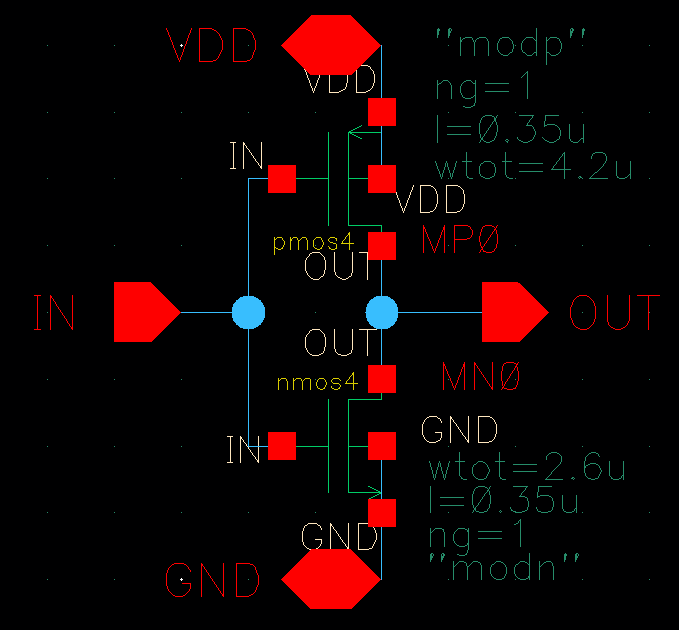
\includegraphics[scale=0.6]{images/schem_inv.png}
    \label{fig:inv_esquematico}
\end{figure}

\begin{figure}[htbp]
    \centering
    \caption{Leiaute do Inversor}
    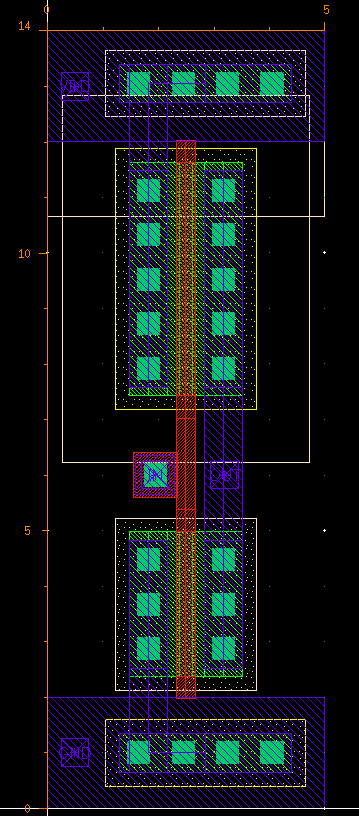
\includegraphics[scale=0.75]{images/layout_inv.png}
    \label{fig:inv_leiaute}
\end{figure}

\begin{figure}[htbp]
    \centering
    \caption{Capacitancias extraídas do leiaute do Inversor}
    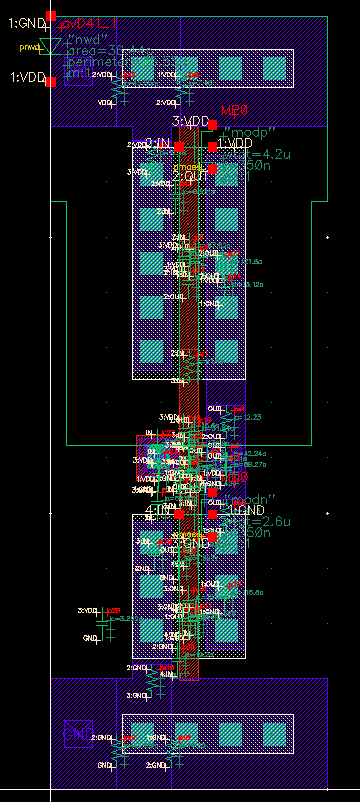
\includegraphics[scale=0.75]{images/extracted_inv.png}
    \label{fig:inv_capacitancias}
\end{figure}

\FloatBarrier

Os resultados da análise transiente desse circuito estão no Capítulo \ref{resultados}.\

A Figura \ref{fig:inv_trans} mostra o esquemático do Inversor na ferramenta \virtuoso, e a Figura \ref{fig:inv_wave} mostra o \textit{waveform} da simulação transiente do mesmo.

\begin{figure}[htbp]
    \centering
    \caption{Esquemático da simulação transiente do Inversor.}
    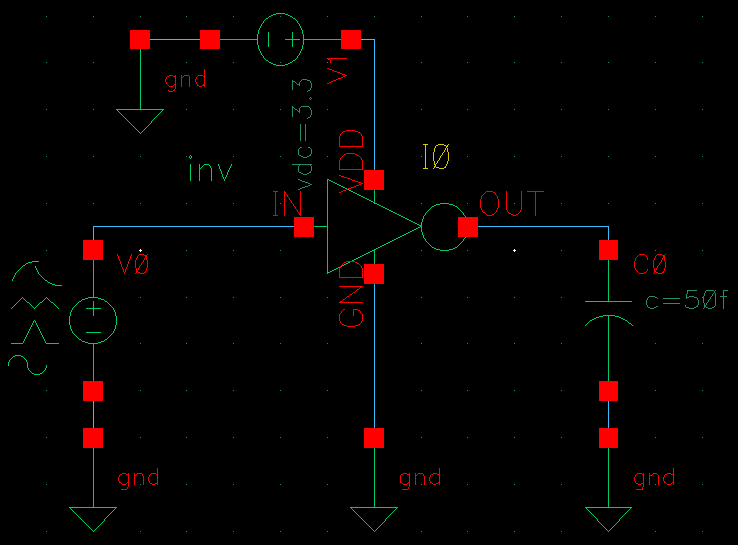
\includegraphics[scale=0.6]{images/schem_inv_trans.png}
    \label{fig:inv_trans}
\end{figure}

\begin{figure}[htbp]
    \centering
    \caption{Waveforms da simulação transiente do Inversor.}
    \label{fig:inv_wave}
    \subfloat[united]{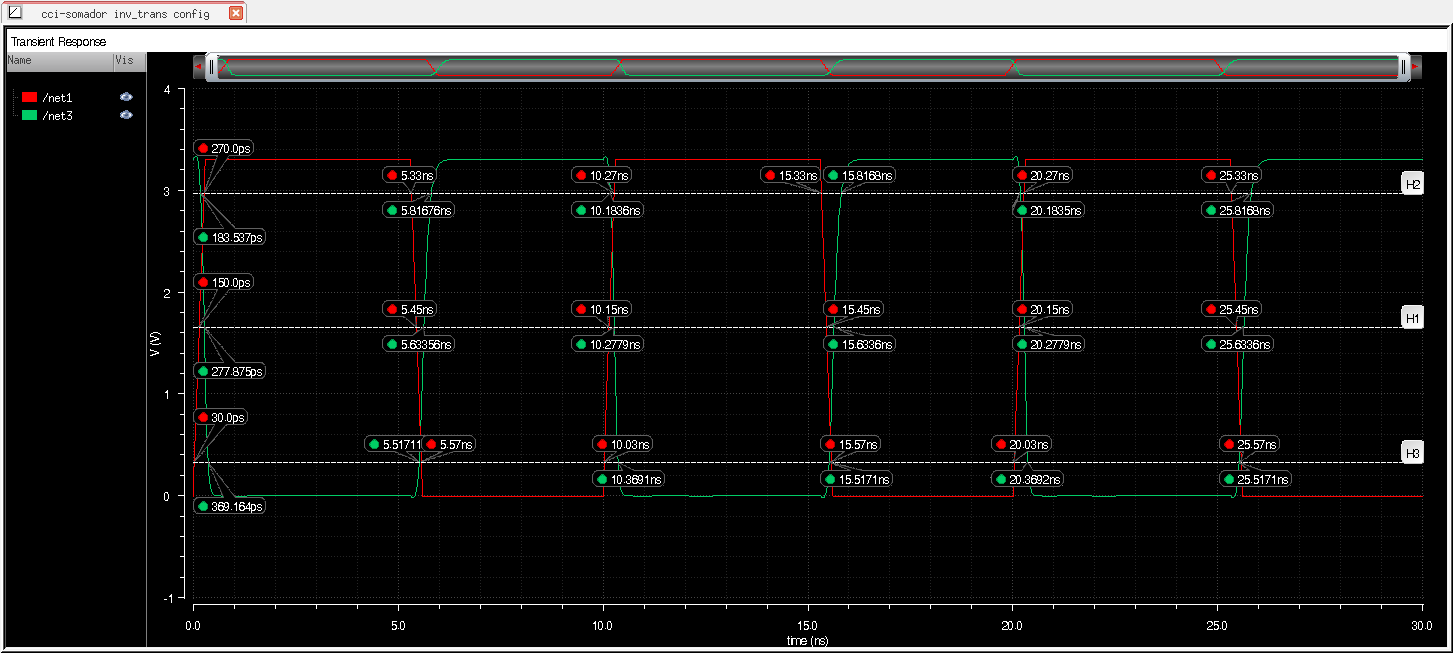
\includegraphics[scale=0.4]{images/wave_inv_united.png}} \\
    \subfloat[separated]{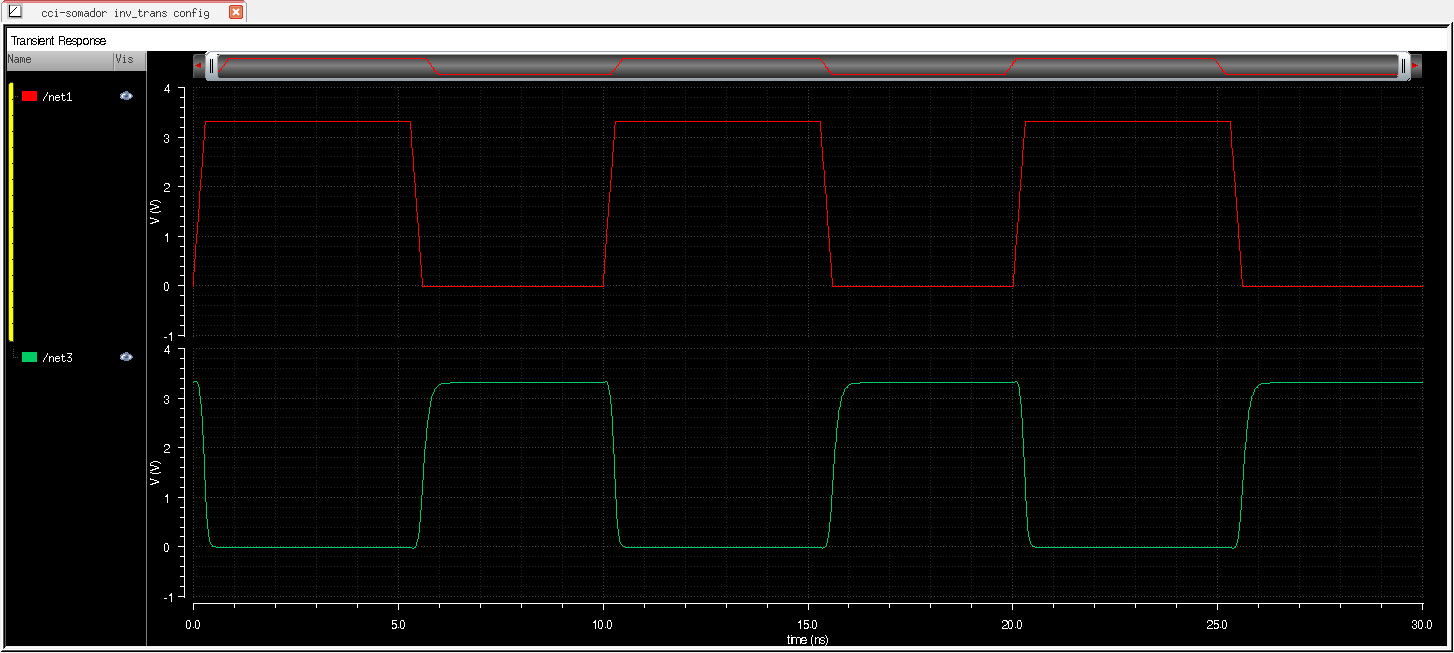
\includegraphics[scale=0.4]{images/wave_inv_sep.png}}
\end{figure}

\FloatBarrier

%%%%%%%%%%%%%%%%%%%%%%%%%%%%%%%%%%%%%%%
%%%%%%%%%%%%%%%%%%%%%%%%%%%%%%%%%%%%%%%

\section{Somador 1 bit}\label{adder_1bit}
O Somador de 1 bit, como visto anteriormente na Tabela \ref{tab:imp}, possuirá transistores PMOS e NMOS dimensionados respectivamente em \SI{4.2}{\um}/\SI{2.1}{\um} e \SI{2.6}{\um}/\SI{1.3}{\um}. 

Essa escolha inusitada de dimensionados de transistores surgiu com a intenção de melhorar a performance da parte do circuito que calcula o \textit{carry-out}, porém, para posicionar esses transistores maiores, tive que realizar o \textit{folding} deles. Essa última decisão ocasionou um roteamento muito mais caótico do que eu previa. Não precisei utilizar camadas mais superiores de metais, quesito onde utilizei, no máximo, a camada de metal 2.

A Figura \ref{fig:1bit_esquematico} mostra o esquemático do Somador na ferramenta \virtuoso, e a Figura \ref{fig:1bit_leiaute} mostra o seu respectivo leiaute.

Como adicional, podemos observar na Figura \ref{fig:1bit_capacitancias} as capacitâncias extraidas do leiaute da Figura \ref{fig:1bit_leiaute}.

\begin{figure}[htbp]
    \centering
    \caption{Esquemático do Somador Completo de 1 bit}
    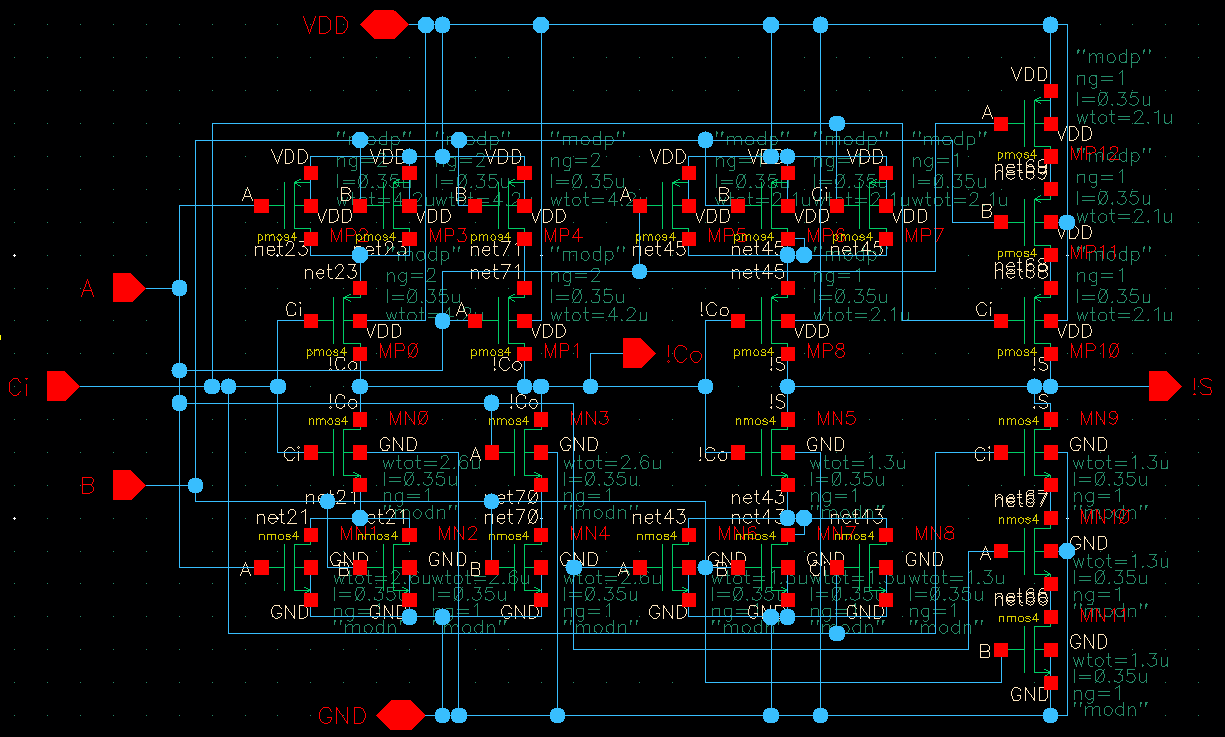
\includegraphics[scale=0.45]{images/schem_1bit.png}
    \label{fig:1bit_esquematico}
\end{figure}

\begin{figure}[htbp]
    \centering
    \caption{Leiaute do Somador Completo de 1 bit}
    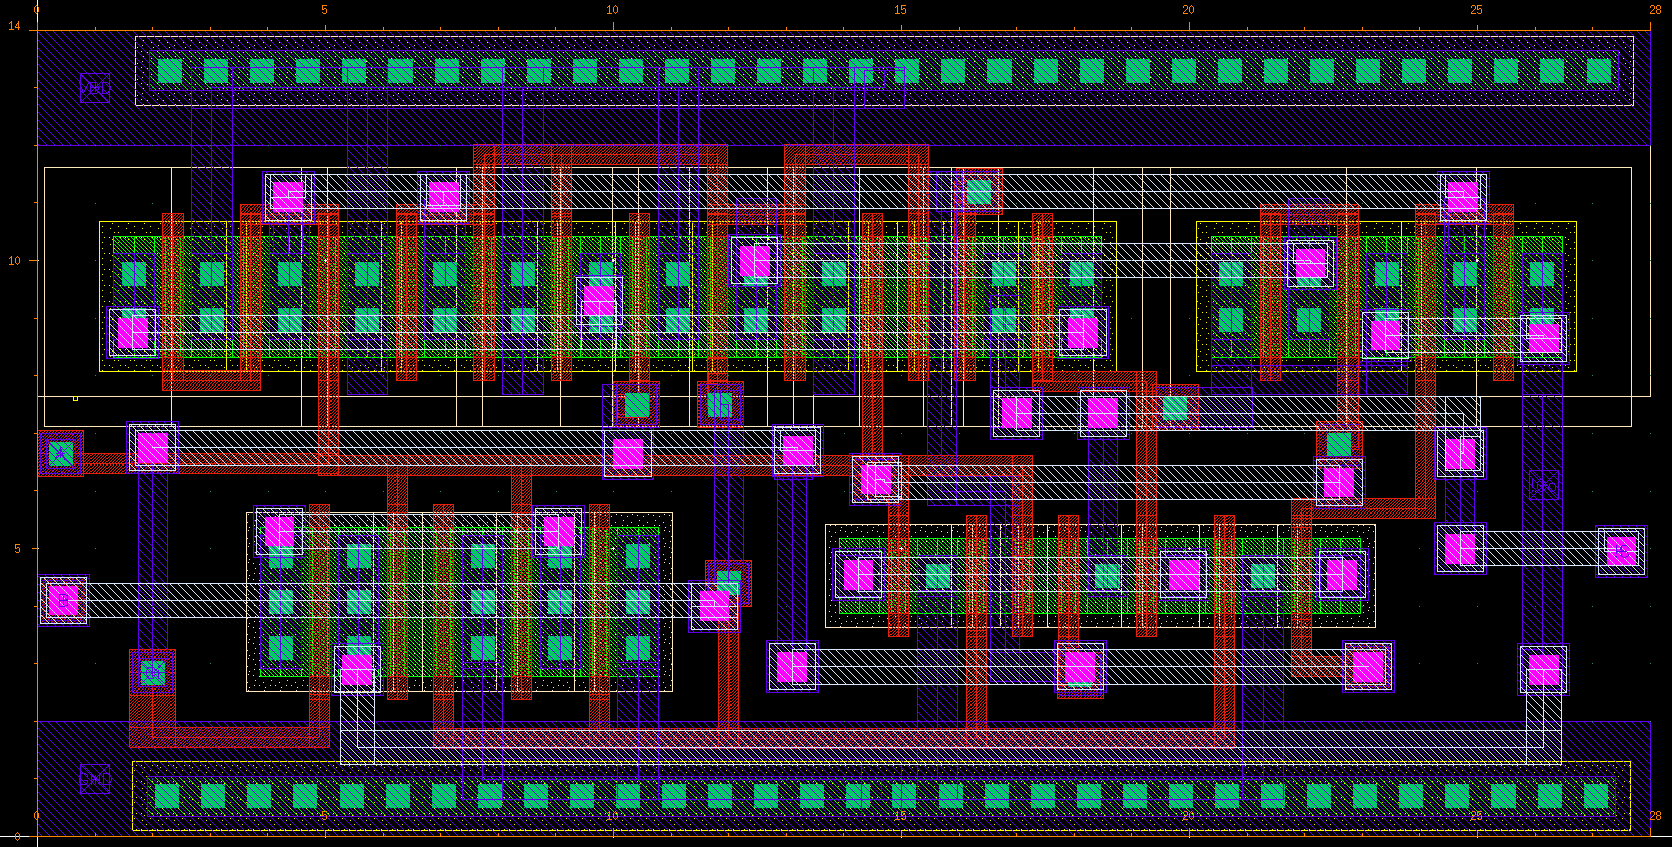
\includegraphics[scale=0.35]{images/layout_1bit.png}
    \label{fig:1bit_leiaute}
\end{figure}

\begin{figure}[htbp]
    \centering
    \caption{Capacitancias extraídas do leiaute do Somador Completo de 1 bit}
    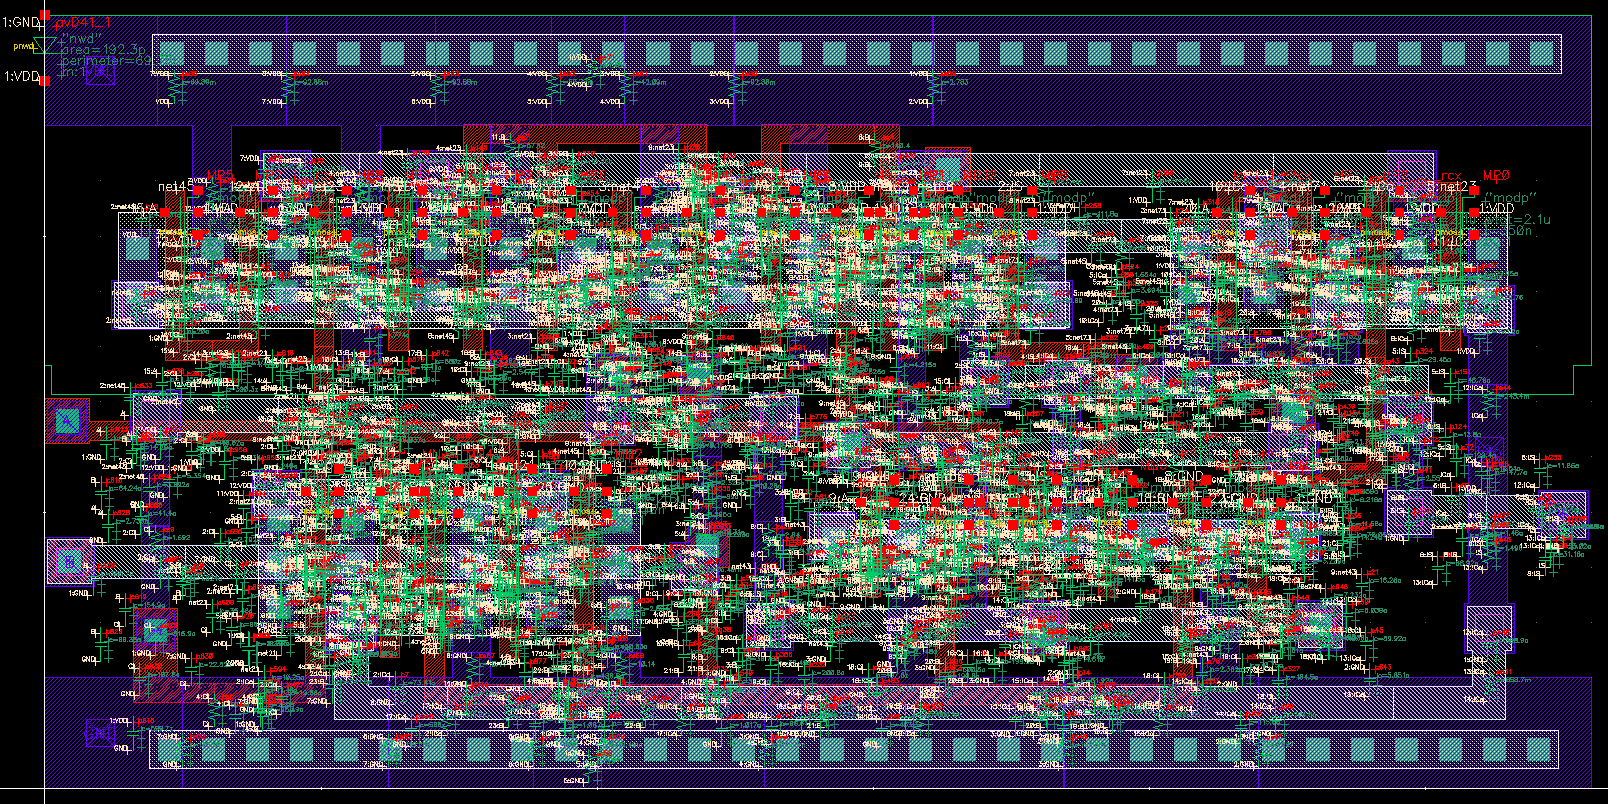
\includegraphics[scale=0.35]{images/extracted_1bit.png}
    \label{fig:1bit_capacitancias}
\end{figure}

\FloatBarrier

Os resultados da análise transiente desse circuito estão no Capítulo \ref{resultados}.

A Figura \ref{fig:1bit_trans} mostra o esquemático do Somador Completo de 1 bit na ferramenta \virtuoso, e a Figura \ref{fig:1bit_wave} mostra o \textit{waveform} da simulação transiente do mesmo.

\begin{figure}[htbp]
    \centering
    \caption{Esquemático da simulação transiente do Somador Completo de 1 bit.}
    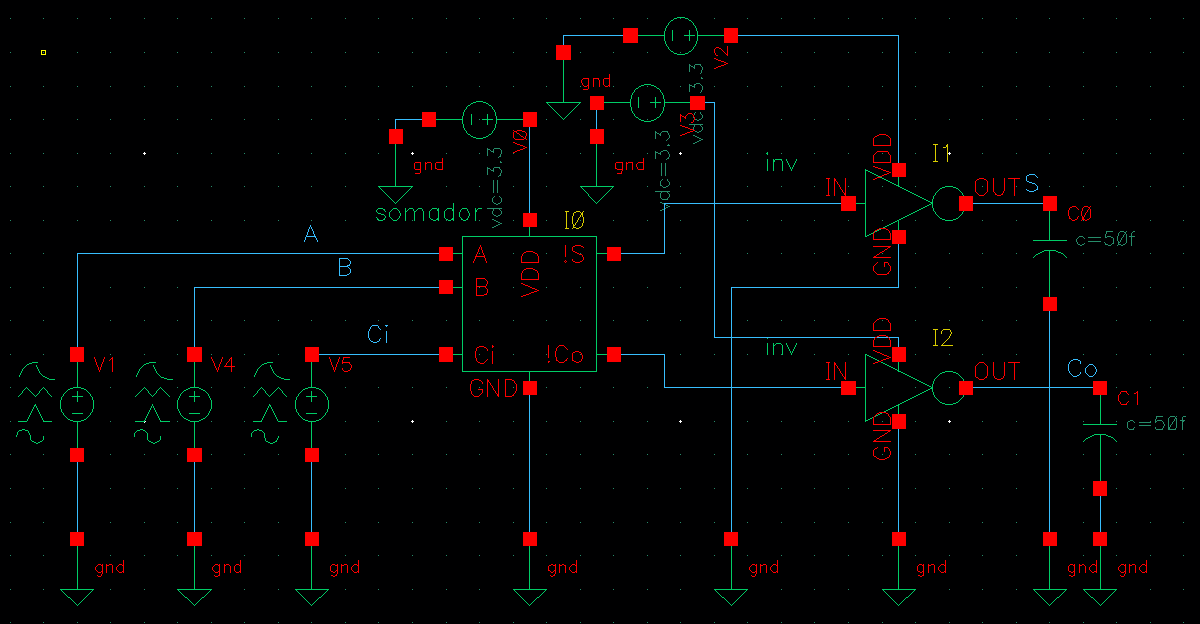
\includegraphics[scale=0.45]{images/schem_1bit_trans.png}
    \label{fig:1bit_trans}
\end{figure}

\begin{figure}[htbp]
    \centering
    \caption{Waveforms da simulação transiente do Somador Completo de 1 bit.}
    \label{fig:1bit_wave}
    \subfloat[united]{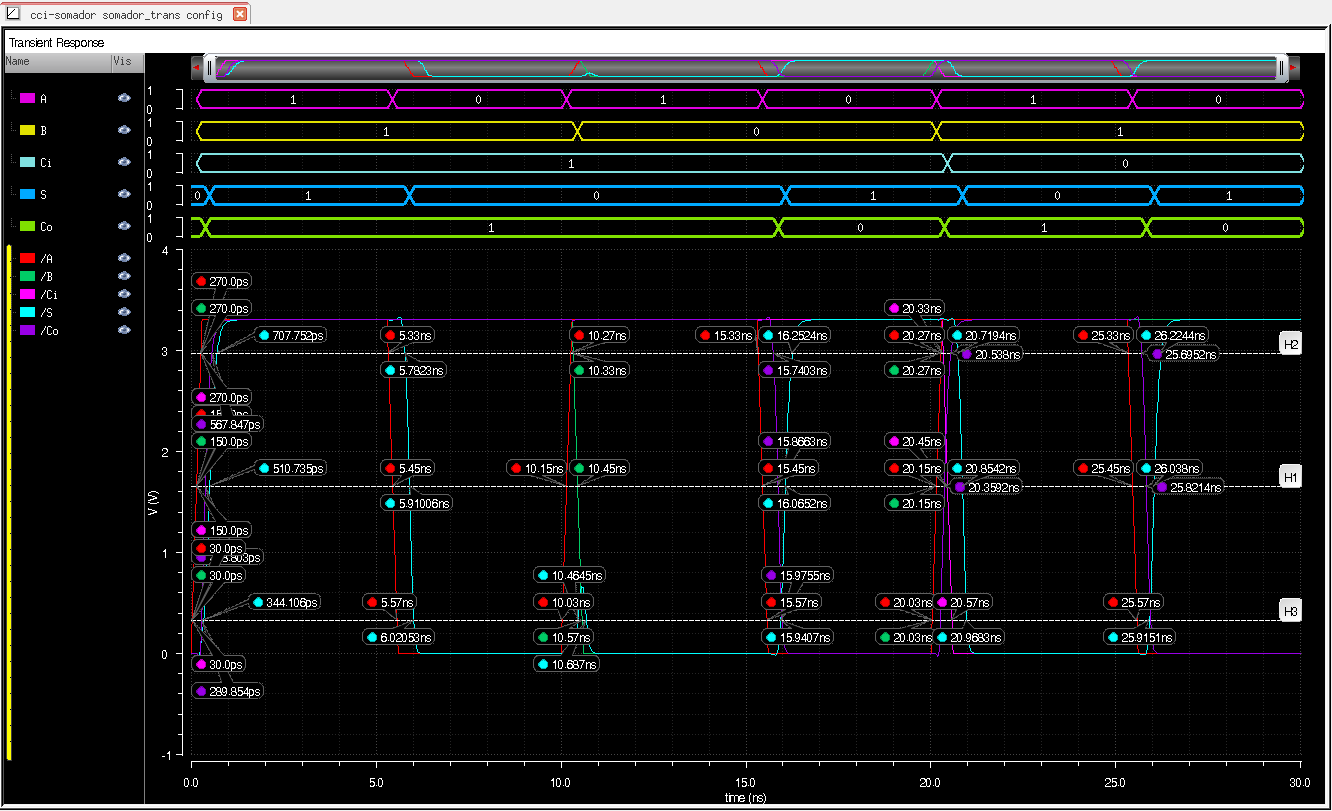
\includegraphics[scale=0.4]{images/wave_1bit_united.png}} \\
    \subfloat[separated]{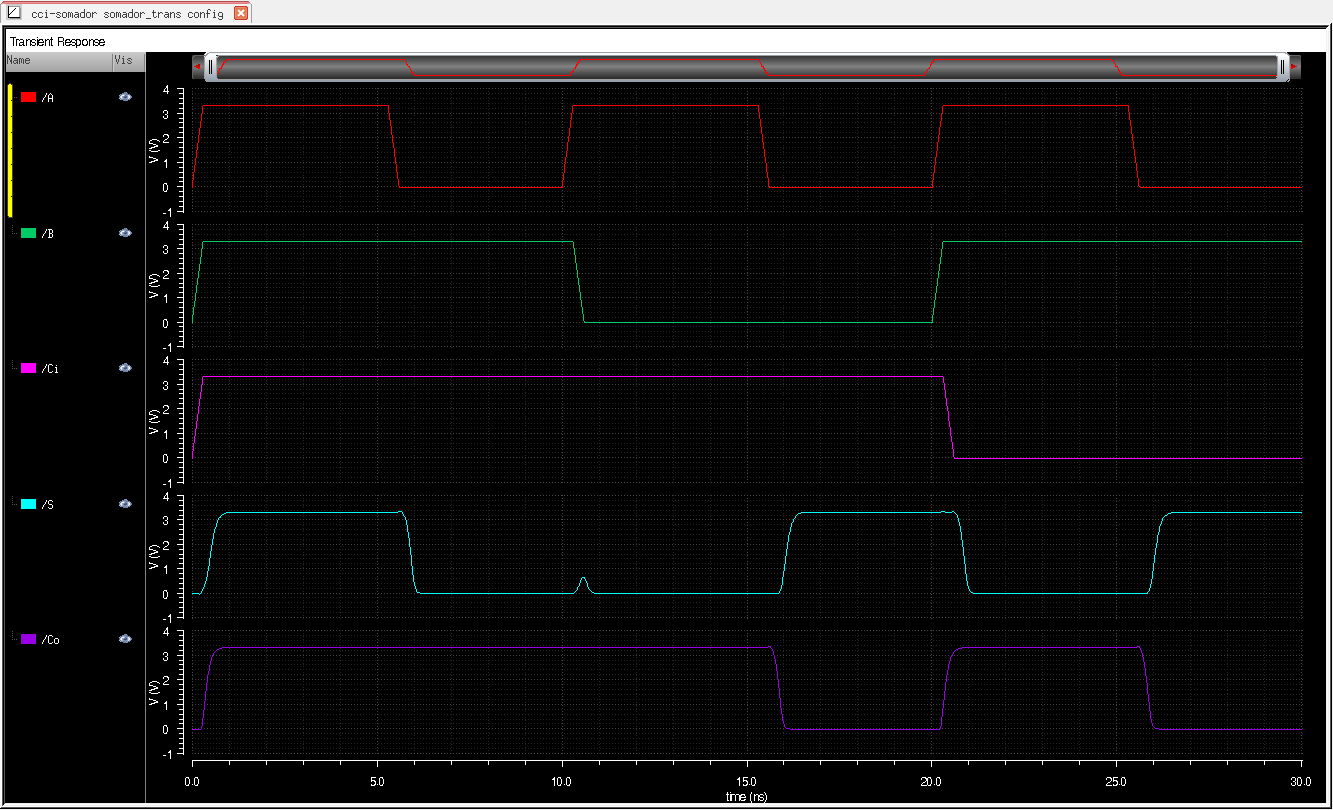
\includegraphics[scale=0.4]{images/wave_1bit_sep.png}}
\end{figure}

\FloatBarrier

%%%%%%%%%%%%%%%%%%%%%%%%%%%%%%%%%%%%%%%%%%%%%%
%%%%%%%%%%%%%%%%%%%%%%%%%%%%%%%%%%%%%%%%%%%%%%

\section{Somador 4 bits}\label{adder_4bit}
O Somador de 4 bits não implementa diretamente nenhum transistor em seu leiaute, sendo um módulo que só utiliza os módulos \ref{adder_1bit} e \ref{inversor}.

A conexão dos módulos foi feita utilizando as camadas de metal 2 e 3. A escolha de ligar os módulos horizontalmente foi ocasionada pela necessidade de rotear algumas trilhas de polisilício sobre as trilhas de alimentação e dreno do Somador de 1 bit, como pode ser observado na Figura \ref{fig:1bit_leiaute}. Sendo assim, eu perdi a oportunidade de aproveitar as trilhas de alimentação organizando os módulos um em cima do outro, como foi demonstrado em aula prática.

A Figura \ref{fig:4bit_esquematico} mostra o esquemático do Inversor na ferramenta \virtuoso, e a Figura \ref{fig:4bit_leiaute} mostra o seu respectivo leiaute.

Como adicional, podemos observar na Figura \ref{fig:4bit_capacitancias} as capacitâncias extraidas do leiaute da Figura \ref{fig:4bit_leiaute}.

\begin{figure}[htbp]
    \centering
    \caption{Esquemático do Somador Completo de 4 bits}
    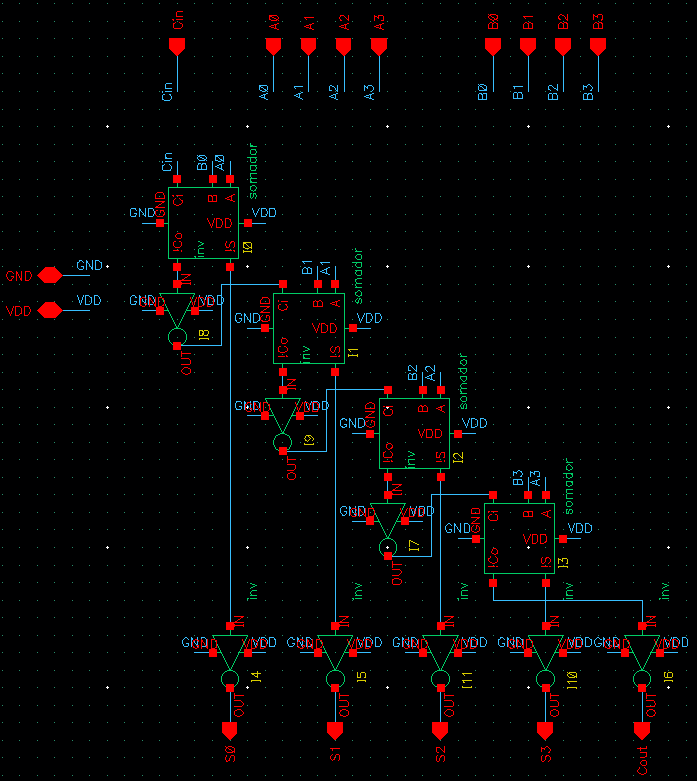
\includegraphics[scale=0.7]{images/schem_4bit.png}
    \label{fig:4bit_esquematico}
\end{figure}

\begin{figure}[htbp]
    \centering
    \caption{Leiaute do Somador Completo de 4 bits}
    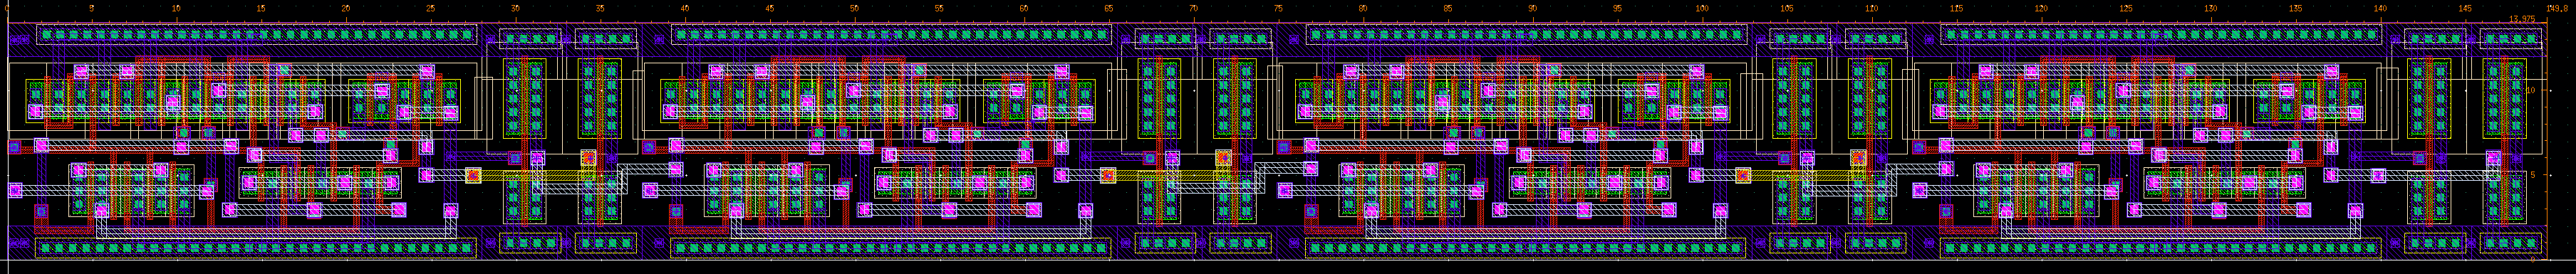
\includegraphics[scale=0.175]{images/layout_4bit.png}
    \label{fig:4bit_leiaute}
\end{figure}

\begin{figure}[htbp]
    \centering
    \caption{Capacitancias extraídas do leiaute do Somador Completo de 4 bits}
    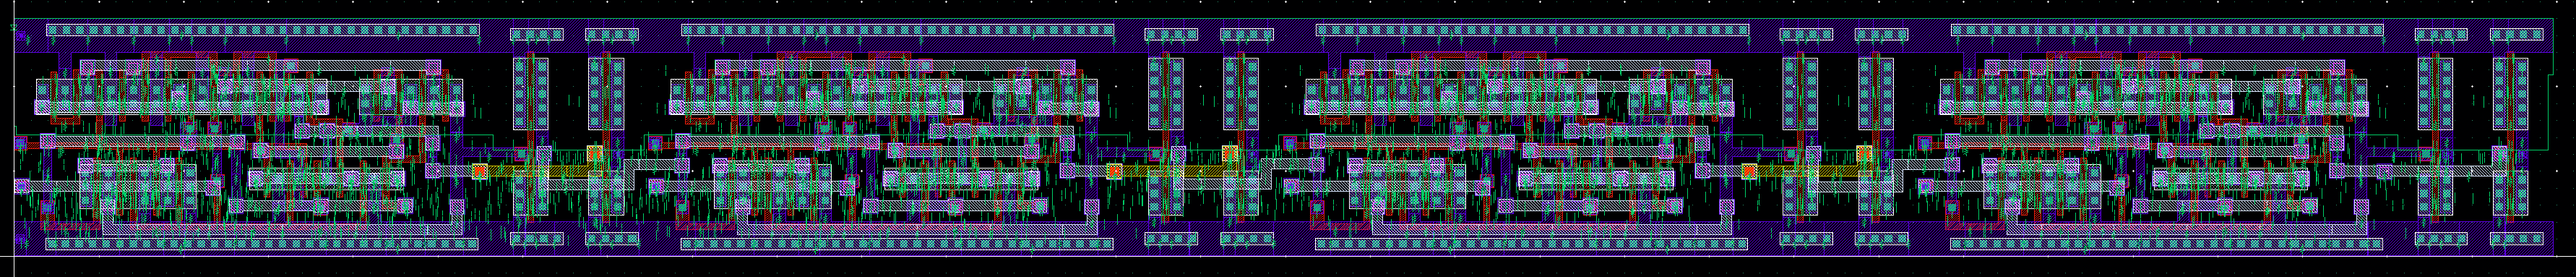
\includegraphics[scale=0.175]{images/extracted_4bit.png}
    \label{fig:4bit_capacitancias}
\end{figure}

\FloatBarrier

Os resultados da análise transiente desse circuito estão no Capítulo \ref{resultados}.\

A Figura \ref{fig:4bit_trans} mostra o esquemático do Somador Completo de 4 bits na ferramenta \virtuoso, e a Figura \ref{fig:4bit_wave} mostra o \textit{waveform} da simulação transiente do mesmo.

\begin{figure}[htbp]
    \centering
    \caption{Esquemático da simulação transiente do Somador Completo de 4 bits.}
    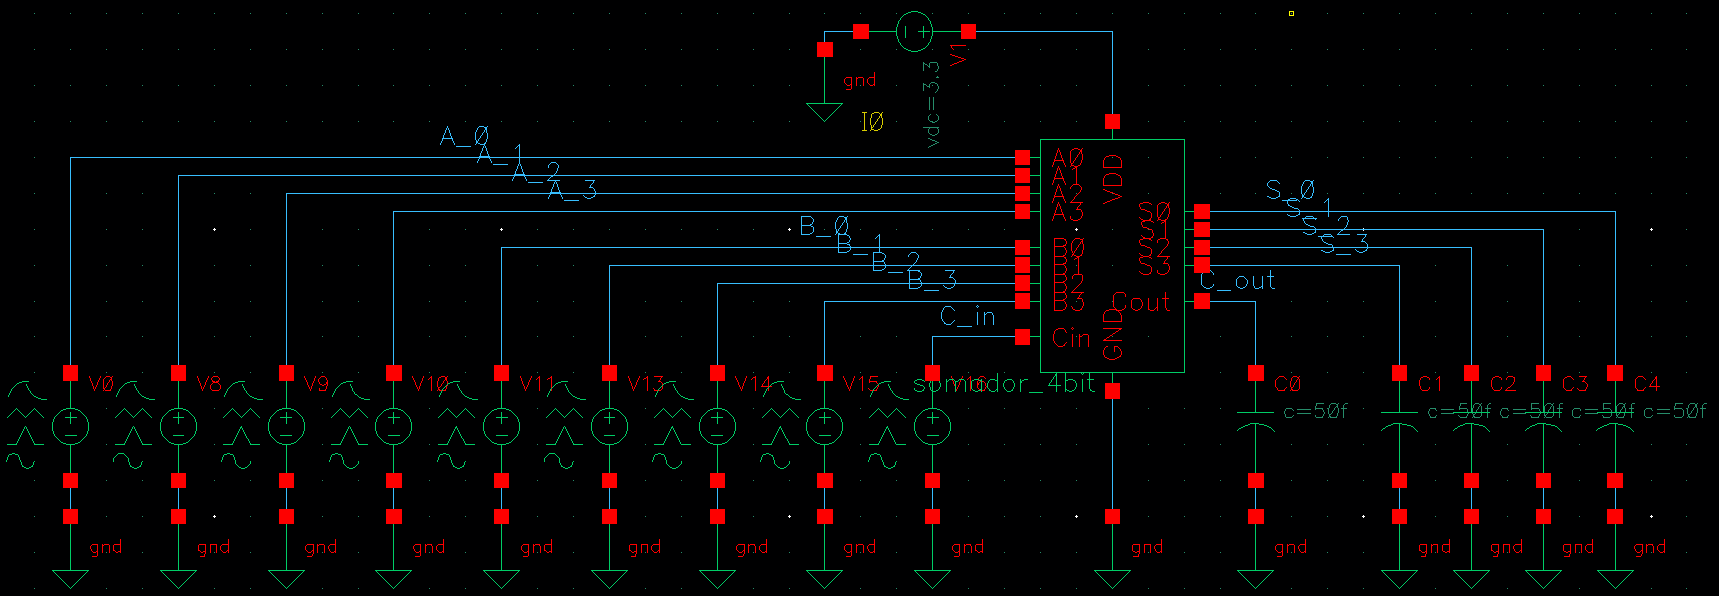
\includegraphics[scale=0.35]{images/schem_4bit_trans.png}
    \label{fig:4bit_trans}
\end{figure}

\begin{figure}[htbp]
    \centering
    \caption{Waveforms da simulação transiente do Somador Completo de 4 bits.}
    \label{fig:4bit_wave}
    \subfloat[united]{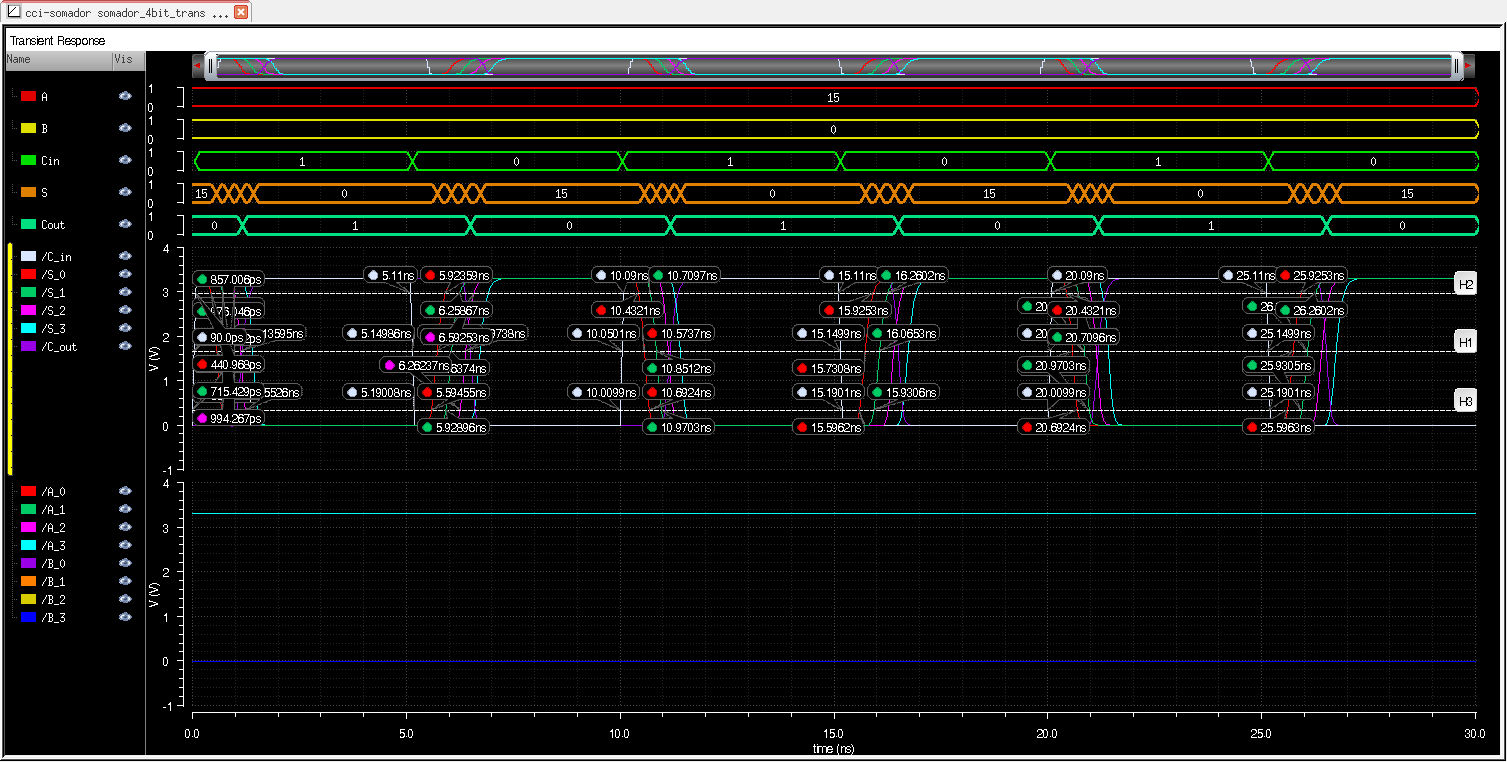
\includegraphics[scale=0.4]{images/wave_4bit_united.png}} \\
    \subfloat[separated]{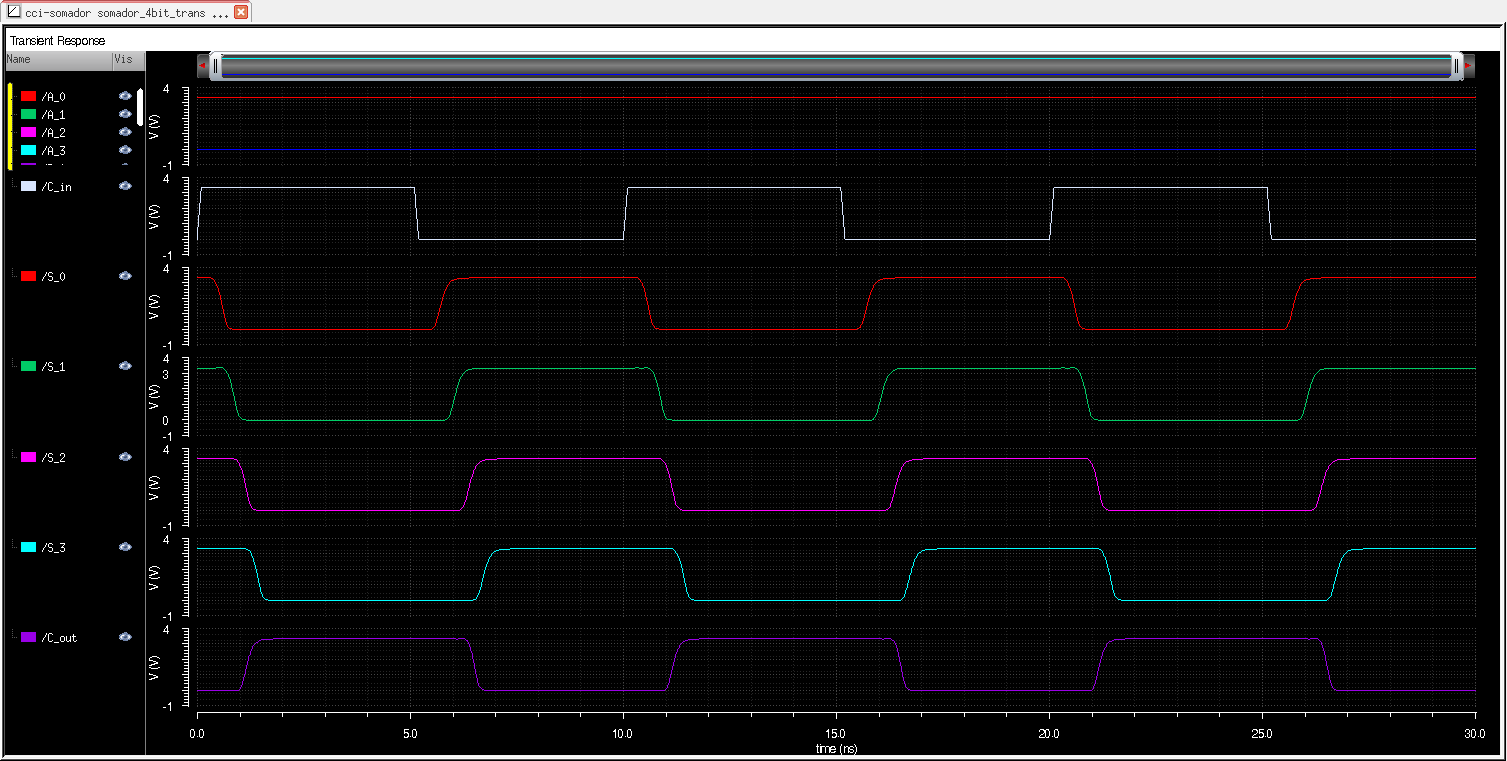
\includegraphics[scale=0.4]{images/wave_4bit_sep.png}}
\end{figure}

\FloatBarrier

\chapter{Resultados}\label{resultados}
Neste capítulo abordaremos os resultados obtidos nas simulações.

\section{Tabela}\label{tabela}
A Tabela \ref{tab:tempo} define os valores encontrados para as métricas temporais definidas no Capítulo \nameref{intro} para os módulos, e a Tabela \ref{tab:potencia} define as métricas de energia e de área para os módulos.

Os dados temporais de propagação coletados para os \textit{carry-out}'s dos somadores foram substituídos, respectivamente, por Tp\textsubscript{LL} e por Tp\textsubscript{HH}. Logo, a propagação média foi, nesses casos, calculada utilizando esses valores.

\begin{table}[ht]
    \centering
    \caption{Resultados temporais das simulações.}
    \small
    \label{tab:tempo}
    \sisetup{round-mode = places, round-precision = 5}
    \begin{tabular}{l l l l l l}
        \hline
        Porta
        & Tp\textsubscript{LH}
        & Tp\textsubscript{HL}
        & Tp\textsubscript{médio}
        & T\textsubscript{LH}
        & T\textsubscript{HL} \\ \hline
        Inversor
        & \SI{0.18356}{\ns} & \SI{0.1279}{\ns} & \SI{0.15573}{\ns} & \SI{0.29965}{\ns}
        & \SI{0.1855}{\ns} \\
        Somador 1 bit (S)
        & \SI{0.588}{\ns} & \SI{0.4042}{\ns} & \SI{0.4961}{\ns} & \SI{0.3117}{\ns}
        & \SI{0.23823}{\ns} \\
        Somador 1 bit (C\textsubscript{out})
        & \SI{0.4163}{\ns} & \SI{0.2092}{\ns} & \SI{0.31275}{\ns} & \SI{0.27799}{\ns}
        & \SI{0.2352}{\ns} \\
        Somador 4 bits (S\textsubscript{3})
        & \SI{1.580881}{\ns} & \SI{1.36019}{\ns} & \SI{1.4705355}{\ns} & \SI{0.328878}{\ns}
        & \SI{0.26146}{\ns} \\
        Somador 4 bits (C\textsubscript{out})
        & \SI{1.354468}{\ns} & \SI{1.12318}{\ns} & \SI{1.238824}{\ns} & \SI{0.31177}{\ns}
        & \SI{0.236881}{\ns} \\
        \hline
    \end{tabular}
\end{table}

\begin{table}[ht]
    \centering
    \caption{Resultados de consumo de potência e de área.}
    \small
    \label{tab:potencia}
    \sisetup{scientific-notation = true, round-mode = places, round-precision = 3}
    \begin{tabular}{l l l l}
        \hline
        $\cdots$
        & P\textsubscript{média}
        & P\textsubscript{RMS}
        & Área \\ \hline
        Inversor 
        & \SI{71.73e-6}{\W} & \SI{335.2e-6}{\W} & \SI{70}{\um\squared}      \\
        Somador 1 bit 
        & \SI{71.07e-6}{\W} & \SI{340.2e-6}{\W} & \SI{392}{\um\squared}     \\
        Somador 4 bits
        & \SI{898.3e-6}{\W} & \SI{1.671e-3}{\W} & \SI{2097.2}{\um\squared}  \\
        \hline
    \end{tabular}
\end{table}

\chapter{Conclusão}

Como conclusões, eu gostaria de comentar sobre as dificuldades que encontrei enquanto fazia os módulos apresentados anteriormente.

Inicialmente, minha maior dificuldade foi o simples dimensionamento dos transistores que decidi que deveriam ser maiores para melhorar a performance do cálculo do bit de \textit{carry-out}. Essa decisão levou a uma complexidade de roteamento consideravelmente maior que eu antecipava. Tive que realizar o \textit{folding} dos transistores PMOS maiores para que fosse possível rotear a célula em primeiro lugar, porém, já que os transistores \textit{folded} não são completamente conectados em seus lados externos, tive problemas ao realizar a verificação LVS, que indicava divergência entre meu esquemático e leiaute. Demorei algum tempo até perceber que eram os transistores dobrados, e quando percebi tive que roteá-los quando necessário, aumentando a quantidade de trilhas de metal 2 na célula. Com isso, utilizar somente as camadas de metal 1 e 2 foi bastante desafiador, e tive que rotear polisilício por cima das trilhas de alimentação.

Por rotear polisilício nas trilhas de alimentação, acabei tendo que mover os pinos de alimentação, o que impossibilitou a união dessas células somadoras num esquema empilhado. Logo, acabei tendo que sequenciar as células horizontalmente, o que deixou o leiaute final muito longo, como se pode observar na Figura \ref{fig:4bit_leiaute}.

Depois disso, tive dificuldades em representar de maneira clara os dados simulados nas waveforms. Após consideráveis tentativas e erros, aprendi a transformar ondas analógicas em sinais digitais para melhor visualização dessa grande quantidade de ondas.

Finalmente, posso afirmar em retrospecto que esse trabalho foi bastante desafiador e combinou todas as atividades vistas na parte prática da disciplina, oferecendo uma janela de perspectiva para os processos de criação de células e leiautes no mercado de trabalho.

%%%%%%%%%%%%%%%%%%%%%%%%%%%%%%%%%%%%%%%%%%%%%%%%%%%%%%%%%%%%%%

%\bibliographystyle{abntex2-alf}
%\bibliography{biblio} 

\end{document}
